\section{How It Works}
\begin{frame}
	\frametitle{How It Detect Lane}
	The autonomous driving uses three ROS nodes to perform the task.
	\begin{itemize}
		\item \texttt{image\_projection}: it project the camera input in order to remove perspective.
		\item \texttt{image\_compensation}: it compensate the projected image. It is used but its effect is null because is not needed compensation in simulation environment.
		\item \texttt{detect\_lane}: it detect the lane. It detect a yellow and a white lane in the projected and compensated image.
		\item \texttt{control\_lane}: it receive an input from \texttt{detect\_lane} and elaborate a \texttt{cmd\_vel} to move the robot in the right direction.
	\end{itemize}
\end{frame}

\begin{frame}
	\frametitle{Camera Input}
	\begin{figure}
		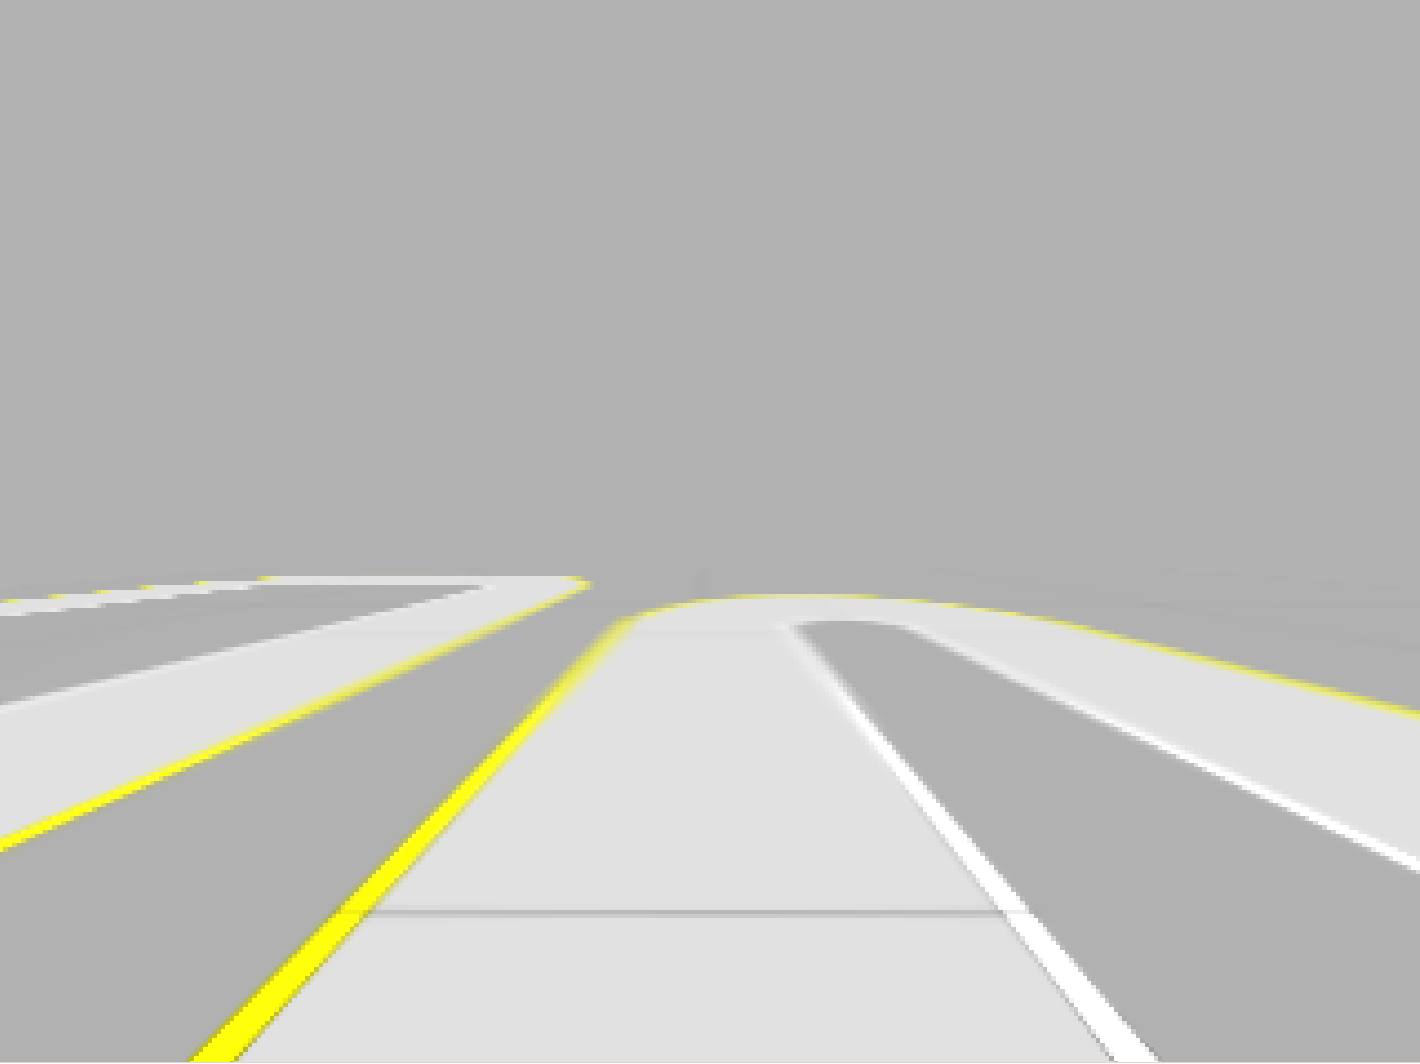
\includegraphics[width=0.7\textwidth]{figures/png/imgraw}
		\caption{Image raw input}
	\end{figure}
\end{frame}

\begin{frame}
	\frametitle{Camera Projection}
	\begin{columns}
	\begin{column}{0.5\textwidth}
	\begin{figure}
		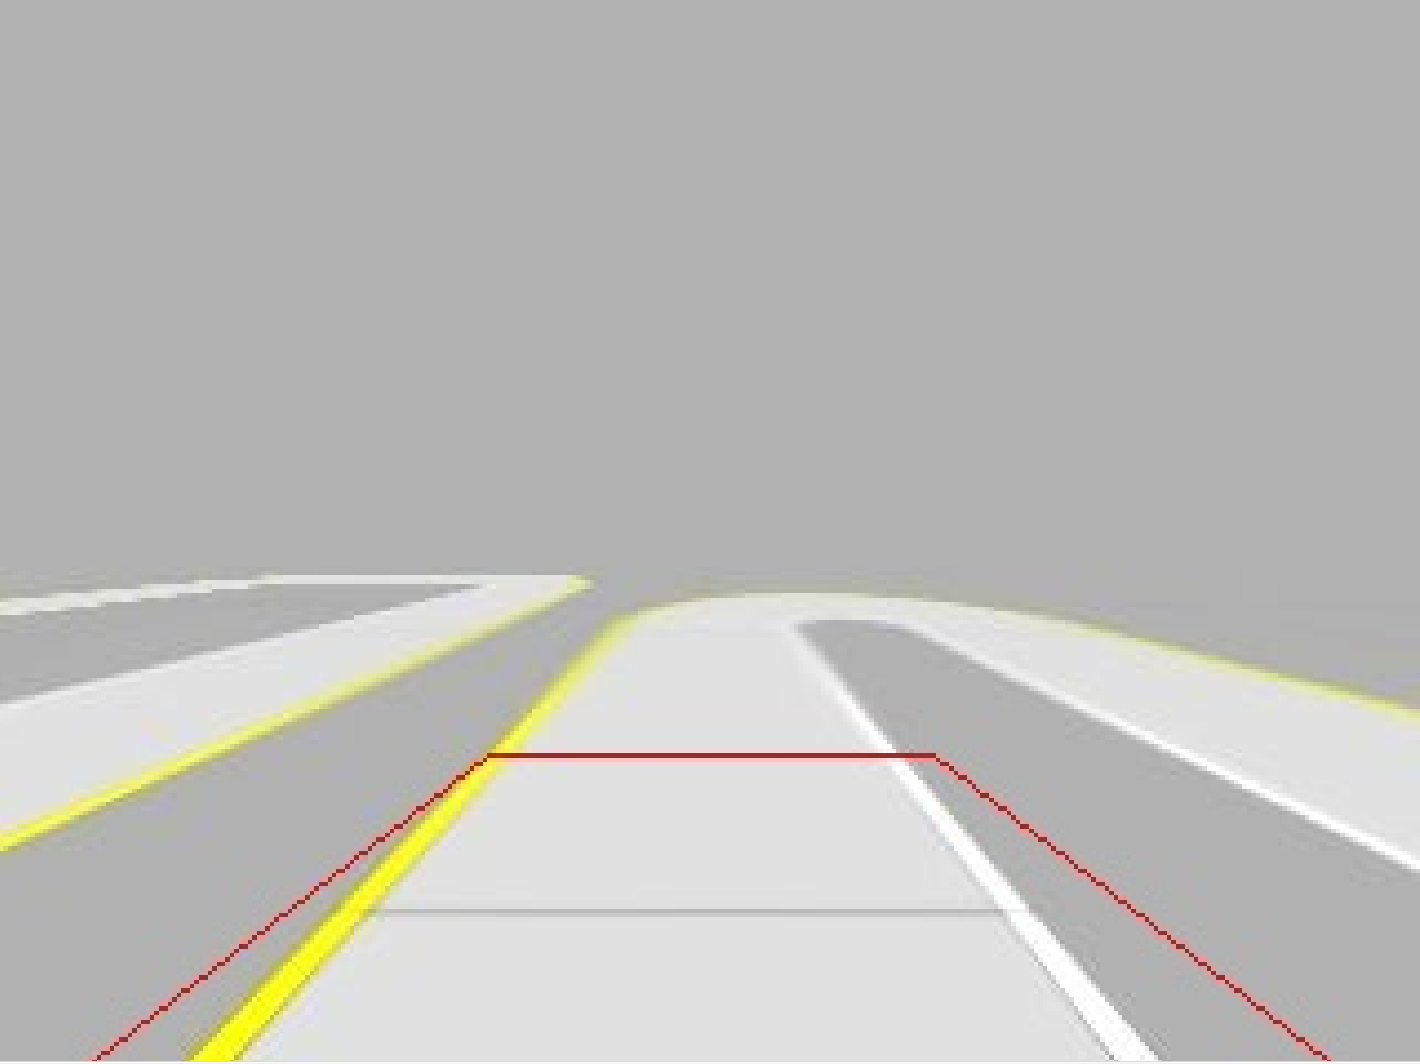
\includegraphics[width=\textwidth]{figures/png/calibprojection}
		\caption{The red box show the area will be projected}
	\end{figure}
	\end{column}
	\begin{column}{0.5\textwidth}
	\begin{figure}
		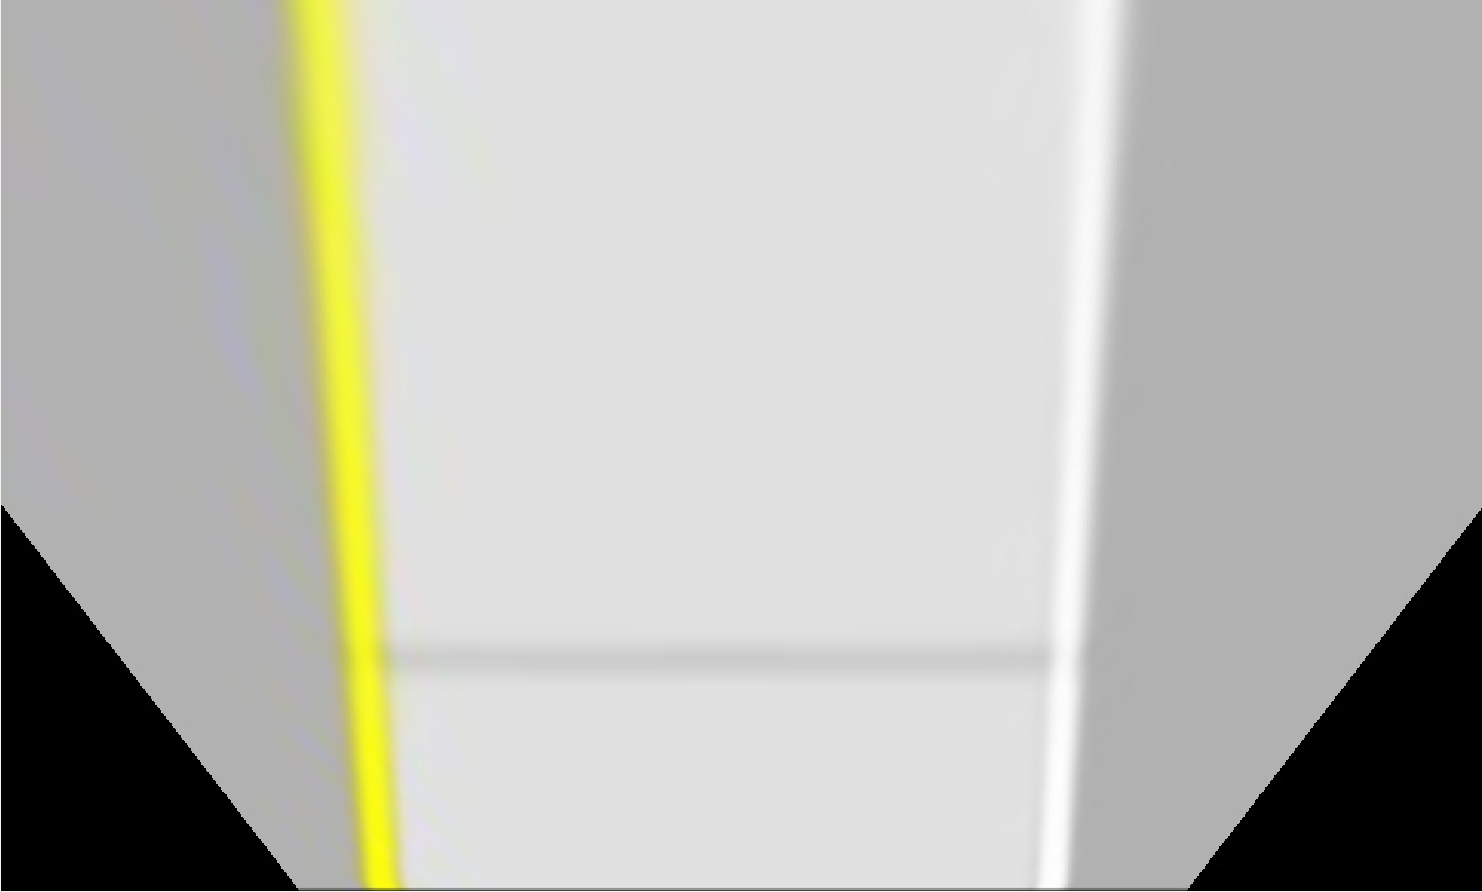
\includegraphics[width=\textwidth]{figures/png/projected}
		\caption{Projected image}
	\end{figure}
	\end{column}
	\end{columns}
\end{frame}

\begin{frame}
	\frametitle{Lane Detection}
	\begin{figure}
		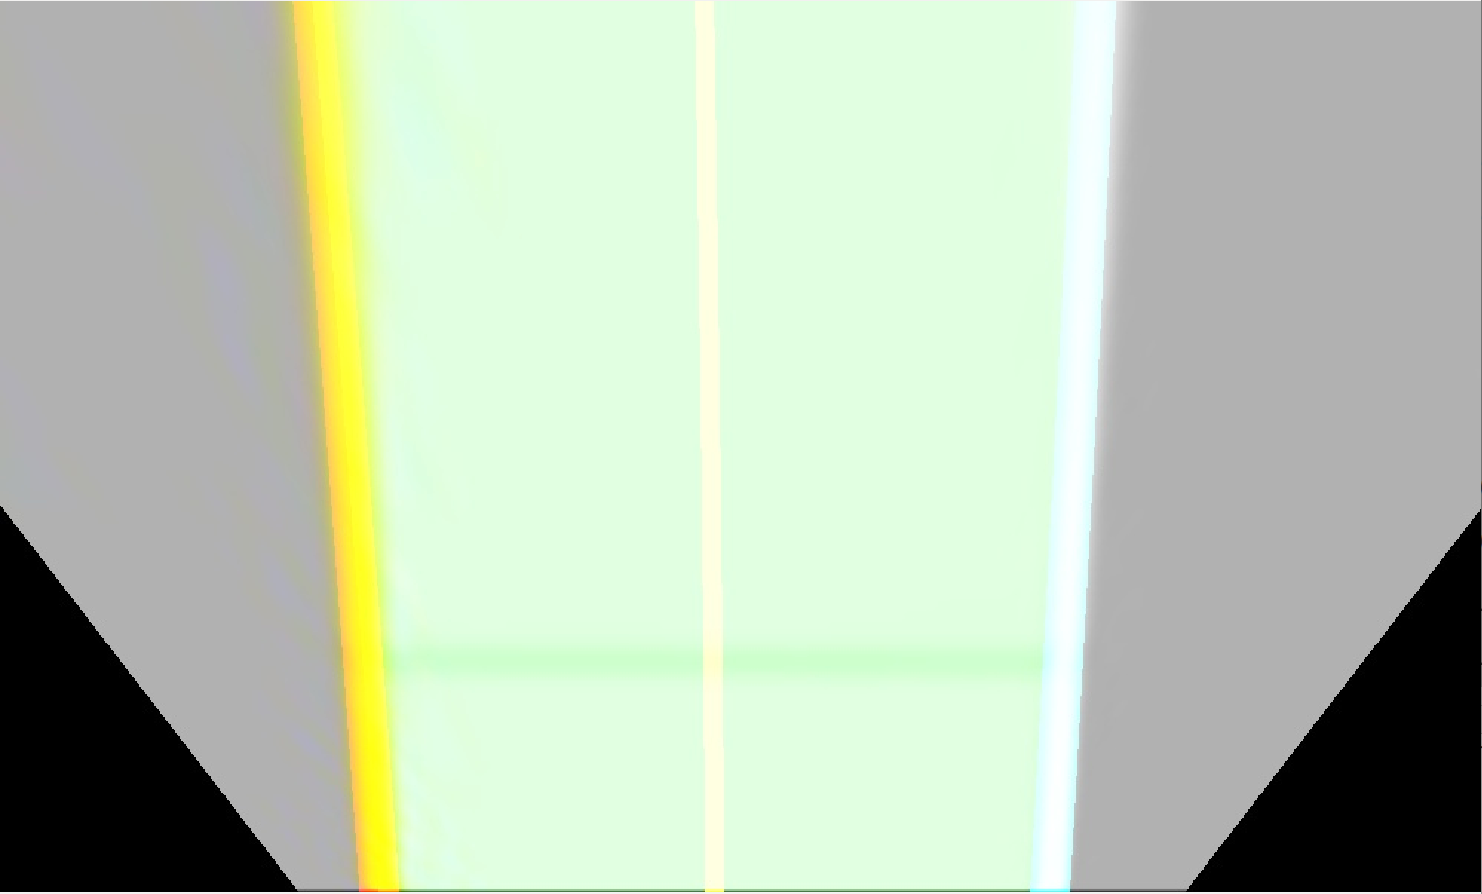
\includegraphics[width=0.7\textwidth]{figures/png/detectlane}
		\caption{Lane Detection}
	\end{figure}
\end{frame}

\begin{frame}
	\frametitle{Graph Representation}
	Below is shown how the nodes communicates:
	\begin{figure}
		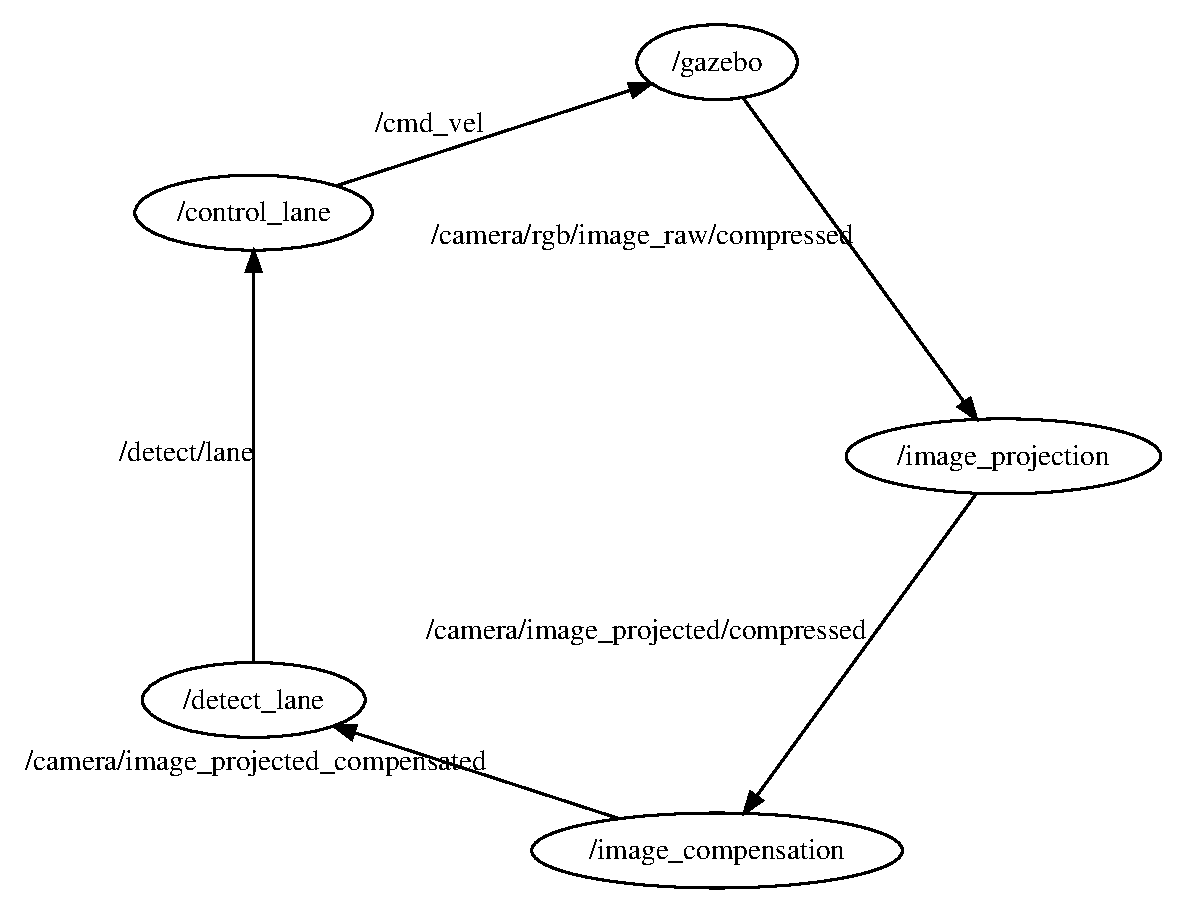
\includegraphics[width=0.7\textwidth]{figures/eps/graph}
	\end{figure}
\end{frame}